% Create a Table of Contents in Beamer
\documentclass[10pt,t]{beamer}
% Theme choice:
\usetheme{Singapore}
\useoutertheme{sidebar}
\usecolortheme{seahorse}
\setbeamercolor{titlelike}{bg=white}
\setbeamercolor{frametitle}{bg=white}
%\setbeamertemplate{frametitle}[default][left]
\setbeamertemplate{navigation symbols}{}

\usepackage{graphicx}
\usepackage{amsmath}
\usepackage{amsfonts}
\usepackage{amssymb}
\usepackage{amsthm}
\usepackage{ulem}
\usepackage{listings}
\usepackage{xcolor}
\usepackage{wrapfig}
\usepackage{subfig}
\usepackage{setspace}
\usepackage{enumerate}
\usepackage{verbatim}
\usepackage{tikz}

% new amber color
\definecolor{amber}{rgb}{1.0, 0.75, 0.0}

% Title page details: 
\title{Bonus Lecture: Spatial Statistics and Under-5 Mortality Estimation} 
\author{Taylor Okonek}
\date{\today}


\begin{document}
	% Title page frame
\begin{frame}
	\titlepage 
\end{frame}


% Outline frame
\begin{frame}{Outline}
	\tableofcontents
\end{frame}

\AtBeginSection[ ]
{
	\begin{frame}{Outline}
		\tableofcontents[currentsection]
	\end{frame}
}


\section{Under-5 Mortality Estimation}

\subsection{Why does this matter?}

\begin{frame}{Millennium Development Goals}
The Millennium Development Goals (MDGs) for the year 2015 were established in 2000 by the United Nations, and aimed to achieve the following:
\vspace{0.3cm}

\begin{enumerate}
	\item To eradicate extreme poverty and hunger
	\item To achieve universal primary education
	\item To promote gender equality and empower women
	\item To reduce child mortality
	\item To improve maternal health
	\item To combat HIV/AIDS, malaria, and other diseases
	\item To ensure environmental sustainability
	\item To develop a global partnership for development
\end{enumerate}
\end{frame}

\begin{frame}{Millennium Development Goals}
The Millennium Development Goals (MDGs) for the year 2015 were established in 2000 by the United Nations, and aimed to achieve the following:
\vspace{0.3cm}

\begin{enumerate}
	\item To eradicate extreme poverty and hunger
	\item To achieve universal primary education
	\item To promote gender equality and empower women
	\item \textcolor{orange}{To reduce child mortality}
	\item To improve maternal health
	\item To combat HIV/AIDS, malaria, and other diseases
	\item To ensure environmental sustainability
	\item To develop a global partnership for development
\end{enumerate} \pause

\end{frame}

\begin{frame}{Millenium Development Goals}
Within each of the eight MDGs, there were specific targets that quantified how each goal would be considered ``met"\dots \pause

\vspace{0.3cm}

\textcolor{blue}{Target 4A: Reduce by two-thirds, between 1990 and 2015, the under-five mortality rate} \pause

\vspace{0.3cm}

In 2004, the United Nations Inter-agency Group for Child Mortality Estimation (\href{https://childmortality.org/}{\textcolor{cyan}{UN IGME}}) was formed to:

\vspace{0.3cm}

\begin{itemize}
	\item assess whether Target 4A (among other within MDG 4) was on track to be met
	\item improve methods for child mortality estimation
	\item share data on child mortality estimates
\end{itemize}

\end{frame}

\begin{frame}{Target 4A}
How did countries do with Target 4A?

\vspace{0.3cm}

Out of 1000 live-births from 1990 to 2015:

\vspace{0.3cm}

\begin{itemize}
	\item Sweden: 6.97 to 2.86 deaths (59\% reduction)
	\item USA: 11.22 to 6.79 deaths (39\% reduction)
	\item Bangladesh: 146.15 to 38.07 deaths (74\% reduction)
	\item Nigeria: 210.05 to 126.45 deaths (40\% reduction)
\end{itemize}



\end{frame}

\begin{frame}{UN IGME Visualizations}
\centering 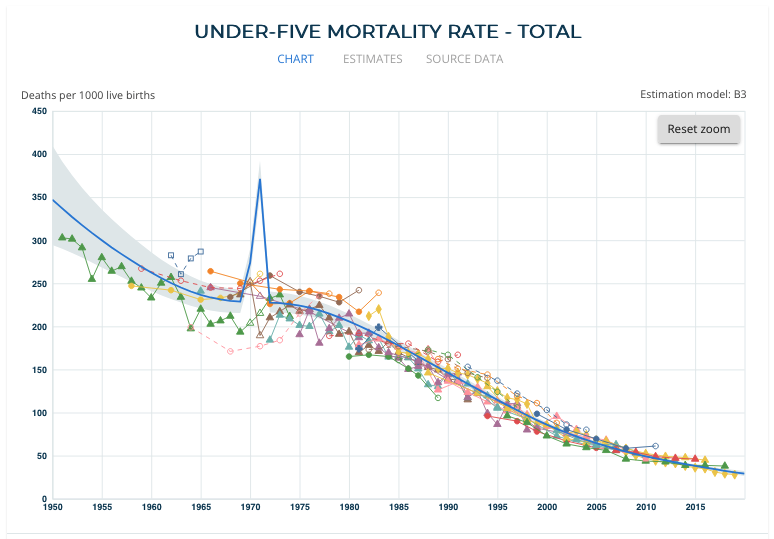
\includegraphics[scale=0.3]{bangladesh_igme.png}
\end{frame}

\begin{frame}{Target 4A}
How did countries do with Target 4A?

\vspace{0.3cm}

Out of 1000 live-births from 1990 to 2015:

\vspace{0.3cm}

\begin{itemize}
	\item Sweden: 6.97 to 2.86 deaths (59\% reduction)
	\item USA: 11.22 to 6.79 deaths (39\% reduction)
	\item Bangladesh: 146.15 to 38.07 deaths (74\% reduction)
	\item Nigeria: 210.05 to 126.45 deaths (40\% reduction)
\end{itemize}

\vspace{0.3cm} 

Progress towards Target 4A varied quite a bit by country, a lot of which had to with valid criticisms of the MDGs as a whole and issues related to financial support received by individual countries from world government organizations.

\end{frame}

\begin{frame}{Sustainable Development Goals}
The MDGs were goals set for 2015, so what about post-2015? 
\vspace{0.3cm}

The UN established the Sustainable Development Goals (SDGs) in 2015 for the target year 2030, to address 17 different goals. These goals are broad and related to one another in some ways, but similar to the MDGs, include specific targets that are meant to be achieved by 2030.

\vspace{0.3cm}

One of the overarching themes of the SDGs (as stated by the UN Secretary General in 2015) is the need for a \textit{Data Revolution for Sustainable Development}. The aim is to improve ``coverage, quality, availability and timeliness of data used to measure and monitor progress toward the SDGs."

\end{frame}

\begin{frame}{Sustainable Development Goals}
SDG 3: Good health and well-being

\vspace{0.3cm}

\begin{itemize}
	\item One of the targets for SDG 3: End all \textcolor{blue}{preventable} deaths of newborns and children under 5 years of age, reduce neonatal mortality to 12 deaths per 1000 live births or lower, and reduce under-5 mortality to 25 deaths per 1000 live births or lower 
\end{itemize}

\vspace{0.3cm}

\pause As of 2021, 195 countries have already met this target. However, UN IGME estimates that if current trends continue, 54 countries will not meet the under-5 mortality target by 2030, and 61 countries will not meet the under-5 mortality target by 2030.

\vspace{0.3cm}

\pause Where can we come in (as biostatisticans) to help countries meet this target, and lower child mortality rates in general?
\end{frame}

\subsection{Why do we need fancy statistical methods?}

\begin{frame}{Child mortality data}
Child mortality data comes in different formats. Just as we've talked in BIOST 311 about different types of study designs, there are also different methods of collecting mortality data!

\vspace{0.3cm}

\begin{itemize}
	\item \textcolor{blue}{Vital registration}: births and deaths are recorded for everyone in a population, including dates for each of these events
	\item \textcolor{blue}{Full birth history}: births and deaths are recorded for a subset of the population, including dates for each of these events
	\item \textcolor{blue}{Summary birth history}: births and deaths are recorded for a subset of the population, but dates are not collected
\end{itemize}

\vspace{0.3cm}

\pause Vital registration data is most complete data on births and deaths that we can have, but \textit{many} low and middle income countries do not have accurate vital registration data. For these countries, we need to estimate mortality rates from full and summary birth histories.
% vital registration, full birth history, summary birth history (census)
% UN IGME reports that almost 2/3 of low and middle income countries have no reliable mortality data in the past three years (this is 2018-2021) (aka no vital registration)
\end{frame}

\begin{frame}{Full and summary birth history data}
Both full and summary birth history data are typically collected via nationally representative surveys, and summary birth history data is often collected in a census as well.

\vspace{0.3cm}

\textcolor{blue}{Summary birth history data}: Mothers are asked how many children they have ever had, and how many of those children have died

\vspace{0.3cm} \pause

\begin{table}[]
	\begin{tabular}{l|l|l|l}
		\multicolumn{1}{c|}{Mother ID} & \multicolumn{1}{c|}{Mother's Age} & \multicolumn{1}{c|}{No. Children} & \multicolumn{1}{c}{No. Died} \\ \hline
		1                              & 16                                & 1                                 & 0                            \\
		2                              & 22                                & 3                                 & 1                            \\
		3                              & 34                                & 4                                 & 2                            \\
		4                              & 18                                & 2                                 & 0                            \\
		5                              & 25                                & 5                                 & 0                           
	\end{tabular}
\end{table}

\pause Summary birth history data is the most \textit{common} source of child mortality information in low and middle income countries, as it is the ``cheapest" to collect.

\end{frame}

\begin{frame}{Full and summary birth history data}
Both full and summary birth history data are typically collected via nationally representative surveys, and summary birth history data is often collected in a census as well.

\vspace{0.3cm}

\textcolor{blue}{Full birth history data}: Mothers are asked how many children they have ever had, as well as their dates of birth and (possibly) death

\vspace{0.3cm} \pause

\begin{table}[]
	\begin{tabular}{l|l|l|l}
		\multicolumn{1}{c|}{Mother ID} & \multicolumn{1}{c|}{Child ID} & \multicolumn{1}{c|}{DOB} & \multicolumn{1}{c}{DOD} \\ \hline
		1                              & 1                             & Jan 2001                 & NA                      \\
		1                              & 2                             & Mar 2003                 & Apr 2003                \\
		2                              & 1                             & Oct 2002                 & NA                      \\
		3                              & 1                             & Feb 2004                 & Sep 2006                \\
		3                              & 2                             & Feb 2005                 & NA                     
	\end{tabular}
\end{table}

\pause Full birth history data is often the most \textit{reliable} source of child mortality information in low and middle income countries, and is what we will focus on in this lecture!

\end{frame}


\begin{frame}{The Demographic and Health Surveys (DHS) Program}
One of the leading sources of full birth history data for low and middle income countries are the Demographic and Health Surveys (DHS). They are designed to provide nationally representative (unbiased) estimates for a variety of demographic indicators. 

\vspace{0.3cm}

As with most surveys, the DHS cannot collect information from every individual in a country. The majority of their surveys to ensure that users of their data are able to make \textit{precise}, unbiased estimates and precictions at the \textcolor{orange}{Administrative 1} level.

\vspace{0.3cm}

\textcolor{orange}{Administrative 1 level}: The largest subnational administrative unit of a country. In the U.S., these are states (and the Administrative 2 level are counties).

\vspace{0.3cm}

\textcolor{blue}{Question:} What do we mean by ensuring precise, unbiased estimates at the Administrative 1 level?

\end{frame}

\begin{frame}{The Demographic and Health Surveys (DHS) Program}
\textcolor{blue}{Question:} What do we mean by ensuring precise, unbiased estimates at the Administrative 1 level?

\vspace{0.3cm}

To get \textbf{unbiased} estimates, we need to assign a weight to each individual in our dataset. The weight for each individual ends up being 1 divided by the probability that they were included in the survey. If we have a simple random sample of individuals, everyone gets an equal weight (this is the simplest case).

\vspace{0.3cm}

To get \textbf{precise} estimates at the Administrative 1 level, we need to have a \textit{large enough} sample size in each Administrative 1 level.

\end{frame}

\begin{frame}{Data sparsity}
Most surveys, including the DHS, are designed to get precise, unbiased estimates at the Administrative 1 level. 

\vspace{0.3cm}

Obtaining \textit{subnational} estimates of quantities like child mortality, disease prevalence, etc. are important for making informed, targeted public health interventions in scenarios where we have limited resources (or decentralized public health infrastructure!)

\vspace{0.3cm}

\textit{However}, public health interventions often take place at the Administrative 2 level. An example of this would be the First Steps program we looked at in Chapter 1, implemented in King County (not the whole state of Washington). In general, estimates at smaller levels of aggregation will be most useful for targeted interventions. 

\vspace{0.3cm}

\pause If we have vital registration data, obtaining reliable estimates at the Administrative 2 level is very straightforward. When we only have access to survey data that is designed to obtain relibale estimates at the Adminstrative 1 level, this gets very complicated very quickly\dots
\end{frame}

\begin{frame}{Data sparsity}

\small To illustrate the issue, suppose we are interested in estimating HIV prevalence at the Administrative 2 level. We collect information on HIV status from a representative sample of individuals. Our survey is designed to get precise estimates at the Administrative 1 level, so our sample size in each Administrative 1 region is large. Each box below represents an Administrative 1 region, and each point represents 1000 people.

\centering
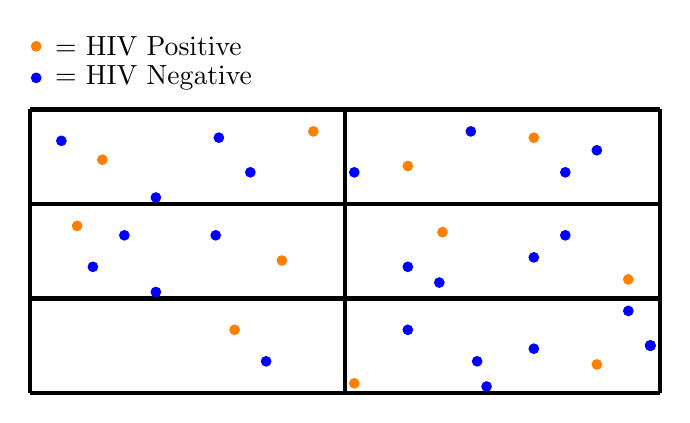
\begin{tikzpicture}[scale=0.4]

\draw[blue,fill=blue] (0.2,12) circle (1ex);
\draw[orange,fill=orange] (0.2,13) circle (1ex);
\node[right] at (0.2,12) {$\text{ = HIV Negative}$};
\node[right] at (0.2,13) {$\text{ = HIV Positive}$};


% Connecting lines LHS
\draw [black, ultra thick] (0,5) -- (20,5);
\draw [black, ultra thick] (0,8) -- (20,8);
\draw [black, ultra thick] (0,11) -- (20,11);
\draw [black, ultra thick] (0,2) -- (20,2);
\draw [black, ultra thick] (0,2) -- (0,11);
\draw [black, ultra thick] (20,2) -- (20,11);
\draw [black, ultra thick] (10,2) -- (10,11);
%\draw [black, ultra thick] (5,2) -- (5,11);
%\draw [black, ultra thick] (15,2) -- (15,11);
% points
\draw[blue,fill=blue] (2,6) circle (1ex);
\draw[blue,fill=blue] (3,7) circle (1ex);
\draw[blue,fill=blue] (4,5.2) circle (1ex);
\draw[blue,fill=blue] (5.9,7) circle (1ex);
\draw[blue,fill=blue] (7,9) circle (1ex);
\draw[blue,fill=blue] (6,10.1) circle (1ex);
\draw[blue,fill=blue] (7.5,3) circle (1ex);
\draw[blue,fill=blue] (1,10) circle (1ex);
\draw[blue,fill=blue] (10.3,9) circle (1ex);
\draw[blue,fill=blue] (12,6) circle (1ex);
\draw[blue,fill=blue] (12,4) circle (1ex);
\draw[blue,fill=blue] (14,10.3) circle (1ex);
\draw[blue,fill=blue] (13,5.5) circle (1ex);
\draw[blue,fill=blue] (14.2,3) circle (1ex);
\draw[blue,fill=blue] (14.5,2.2) circle (1ex);
\draw[blue,fill=blue] (16,3.4) circle (1ex);
\draw[blue,fill=blue] (17,9) circle (1ex);
\draw[blue,fill=blue] (18,9.7) circle (1ex);
\draw[blue,fill=blue] (19,4.6) circle (1ex);
\draw[blue,fill=blue] (19.7,3.5) circle (1ex);
\draw[blue,fill=blue] (19.7,3.5) circle (1ex);
\draw[blue,fill=blue] (19.7,3.5) circle (1ex);
\draw[blue,fill=blue] (19.7,3.5) circle (1ex);
\draw[blue,fill=blue] (17,7) circle (1ex);
\draw[blue,fill=blue] (16,6.3) circle (1ex);
\draw[blue,fill=blue] (4, 8.2) circle (1ex);

\draw[orange,fill=orange] (1.5,7.3) circle (1ex);
\draw[orange,fill=orange] (8,6.2) circle (1ex);
\draw[orange,fill=orange] (2.3,9.4) circle (1ex);
\draw[orange,fill=orange] (9,10.3) circle (1ex);
\draw[orange,fill=orange] (12,9.2) circle (1ex);
\draw[orange,fill=orange] (16,10.1) circle (1ex);
\draw[orange,fill=orange] (13.1,7.1) circle (1ex);
\draw[orange,fill=orange] (19,5.6) circle (1ex);
\draw[orange,fill=orange] (6.5,4) circle (1ex);
\draw[orange,fill=orange] (10.3,2.3) circle (1ex);
\draw[orange,fill=orange] (18,2.9) circle (1ex);

\end{tikzpicture}
\end{frame}

\begin{frame}{Data sparsity}

\small We had a reasonable number of observations in each Administrative 1 region on the previous slide, but if we now split our ``map" into Administrative 2 regions, we can see that one of our Administrative 2 regions has no data! How do we make reasonable, precise estimates for Administrative 2 regions with little to no data? \textcolor{blue}{This is where statistics comes in!}

\centering
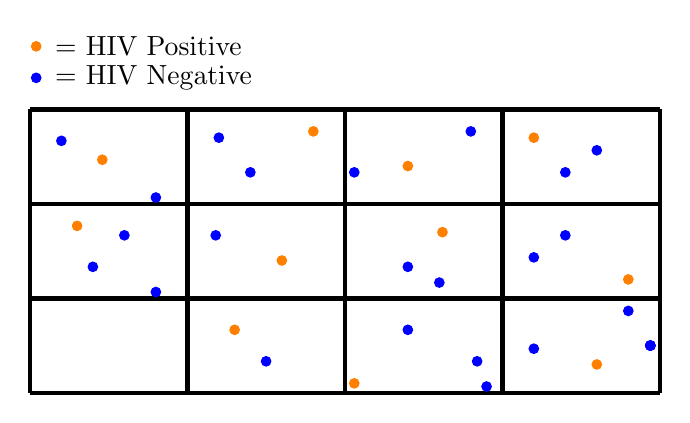
\begin{tikzpicture}[scale=0.4]

\draw[blue,fill=blue] (0.2,12) circle (1ex);
\draw[orange,fill=orange] (0.2,13) circle (1ex);
\node[right] at (0.2,12) {$\text{ = HIV Negative}$};
\node[right] at (0.2,13) {$\text{ = HIV Positive}$};


% Connecting lines LHS
\draw [black, ultra thick] (0,5) -- (20,5);
\draw [black, ultra thick] (0,8) -- (20,8);
\draw [black, ultra thick] (0,11) -- (20,11);
\draw [black, ultra thick] (0,2) -- (20,2);
\draw [black, ultra thick] (0,2) -- (0,11);
\draw [black, ultra thick] (20,2) -- (20,11);
\draw [black, ultra thick] (10,2) -- (10,11);
\draw [black, ultra thick] (5,2) -- (5,11);
\draw [black, ultra thick] (15,2) -- (15,11);
% points
\draw[blue,fill=blue] (2,6) circle (1ex);
\draw[blue,fill=blue] (3,7) circle (1ex);
\draw[blue,fill=blue] (4,5.2) circle (1ex);
\draw[blue,fill=blue] (5.9,7) circle (1ex);
\draw[blue,fill=blue] (7,9) circle (1ex);
\draw[blue,fill=blue] (6,10.1) circle (1ex);
\draw[blue,fill=blue] (7.5,3) circle (1ex);
\draw[blue,fill=blue] (1,10) circle (1ex);
\draw[blue,fill=blue] (10.3,9) circle (1ex);
\draw[blue,fill=blue] (12,6) circle (1ex);
\draw[blue,fill=blue] (12,4) circle (1ex);
\draw[blue,fill=blue] (14,10.3) circle (1ex);
\draw[blue,fill=blue] (13,5.5) circle (1ex);
\draw[blue,fill=blue] (14.2,3) circle (1ex);
\draw[blue,fill=blue] (14.5,2.2) circle (1ex);
\draw[blue,fill=blue] (16,3.4) circle (1ex);
\draw[blue,fill=blue] (17,9) circle (1ex);
\draw[blue,fill=blue] (18,9.7) circle (1ex);
\draw[blue,fill=blue] (19,4.6) circle (1ex);
\draw[blue,fill=blue] (19.7,3.5) circle (1ex);
\draw[blue,fill=blue] (19.7,3.5) circle (1ex);
\draw[blue,fill=blue] (19.7,3.5) circle (1ex);
\draw[blue,fill=blue] (19.7,3.5) circle (1ex);
\draw[blue,fill=blue] (17,7) circle (1ex);
\draw[blue,fill=blue] (16,6.3) circle (1ex);
\draw[blue,fill=blue] (4, 8.2) circle (1ex);

\draw[orange,fill=orange] (1.5,7.3) circle (1ex);
\draw[orange,fill=orange] (8,6.2) circle (1ex);
\draw[orange,fill=orange] (2.3,9.4) circle (1ex);
\draw[orange,fill=orange] (9,10.3) circle (1ex);
\draw[orange,fill=orange] (12,9.2) circle (1ex);
\draw[orange,fill=orange] (16,10.1) circle (1ex);
\draw[orange,fill=orange] (13.1,7.1) circle (1ex);
\draw[orange,fill=orange] (19,5.6) circle (1ex);
\draw[orange,fill=orange] (6.5,4) circle (1ex);
\draw[orange,fill=orange] (10.3,2.3) circle (1ex);
\draw[orange,fill=orange] (18,2.9) circle (1ex);

\end{tikzpicture}
\end{frame}

\begin{frame}{Summary}
Little to not data in small areas (in this case, Administrative 2 regions) occurs all the time!

\vspace{0.3cm}

We \textit{need} estimates in all Administrative 2 regions in order to inform targeted interventions. In addition, countries use these subnational estimates to measure their own progress towards a variety of SDGs (not just under-5 mortality!).

\vspace{0.3cm}

Where statistics can help us is through making \textit{reasonable} assumptions about the spatial structure of our data, to allow us to estimate under-5 mortality in \textit{all} Administrative 2 regions with a high enough precision to be practically useful.
\end{frame}

\section{Spatial Statistics}

\begin{frame}{Spatial statistics}
Spatial statistics is an \textit{incredibly} broad subfield of statistics, and we will only touch on a small part of it in this lecture. In particular, we will focus on \textcolor{blue}{discrete} spatial statistics.
\end{frame}

\subsection{Dependent data}

\subsection{Bayesian statistics}

\section{Cool maps and open statistical questions}


\end{document}